%% Time-stamp: <2018-10-18 20:24:12 (marc)>
\documentclass[xcolor=x11names,compress, mathserif]{beamer}

\newcommand{\hackspace}{\hspace{4.2mm}}
\newcommand{\showstudent}[1]{}
\newcommand\hmmax{0}
\newcommand\bmmax{0}





% talk/author information
\newcommand{\authorname}{Yingzhen Li}
\newcommand{\authoremail}{yingzhen.li@imperial.ac.uk}
\newcommand{\authortwitter}{liyzhen2}
\newcommand{\authoraffiliation}{
  Department of Computing\\Imperial
  College London}
\newcommand{\slidesettitle}{\imperialBlue{Probabilistic PCA}}
\newcommand{\footertitle}{Probabilistic PCA}
\newcommand{\location}{Imperial College London}
\newcommand{\talkDate}{Nov 25, 2022}



\date{\imperialGray{\talkDate}}




% load defaults
%\usepackage{../MarkMathCmds}
\input{../includes/header.tex}
\input{../includes/YingzhenNotations.tex}
\newcommand{\BW}{\mathbf{W}}
\newcommand{\BC}{\mathbf{C}}


\input{../includes/titlepage.tex}
\linespread{1.2}


\begin{frame}{PCA: Recap}
Motivation: real-world data $\mathcal{D} = \{ \x_n \}_{n=1}^N, \x_n \in \mathbb{R}^{D \times 1}$ often lies in a lower-dimensional space

PCA's idea to ``save memory'':
\begin{itemize}
\item Project $\x_n$ onto a lower-dim space $span(\{\Bb_1, ..., \Bb_M\})$ to get
$$\z_n := (z_{n1}, ..., z_{nM}), \quad z_{nm} = \Bb_m, \quad M < D, $$
then store $\z_n$ instead of $\x_n$;
\item When needed, get reconstruction $\tilde{\x}_n = \sum_{m=1}^M z_{nm} \Bb_m$
\item To get orthonormal basis $\{\Bb_1, ..., \Bb_M\}$: PCA
\begin{itemize}
	\item maximum variance view
	\item minimum reconstruction error view
\end{itemize}
\end{itemize}

\end{frame}

\begin{frame}{PCA: Recap}

\begin{figure}
\centering
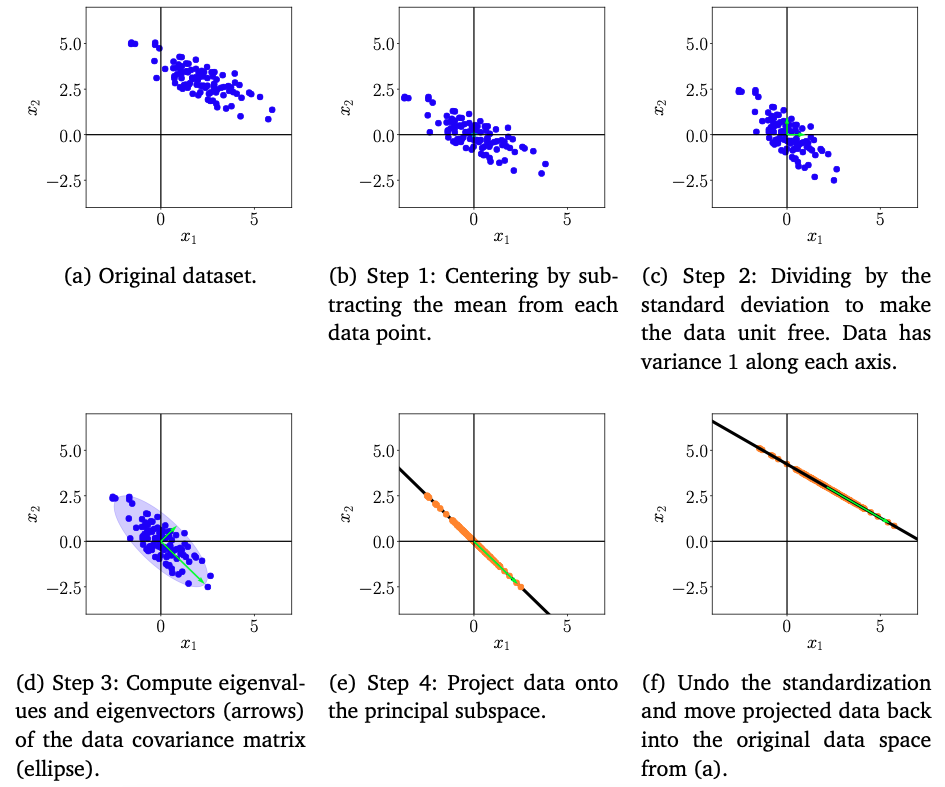
\includegraphics[width=0.7\linewidth]{figures-pca/keysteps_pca.png}
\end{figure}
\hfill \tiny{Fig from the MML book.}

\end{frame}

\begin{frame}{PCA: Recap}
An issue with PCA in test time:
\begin{itemize}
\item Given an $\x$, we can find the low-dim projection $\z$ of it using trained PCA
\item However, PCA alone cannot generate new $\x$ (unless we do something further)
\end{itemize}

\end{frame}

\begin{frame}{Generative models}
To name a few dimensionality reduction methods:

\begin{figure}
\centering
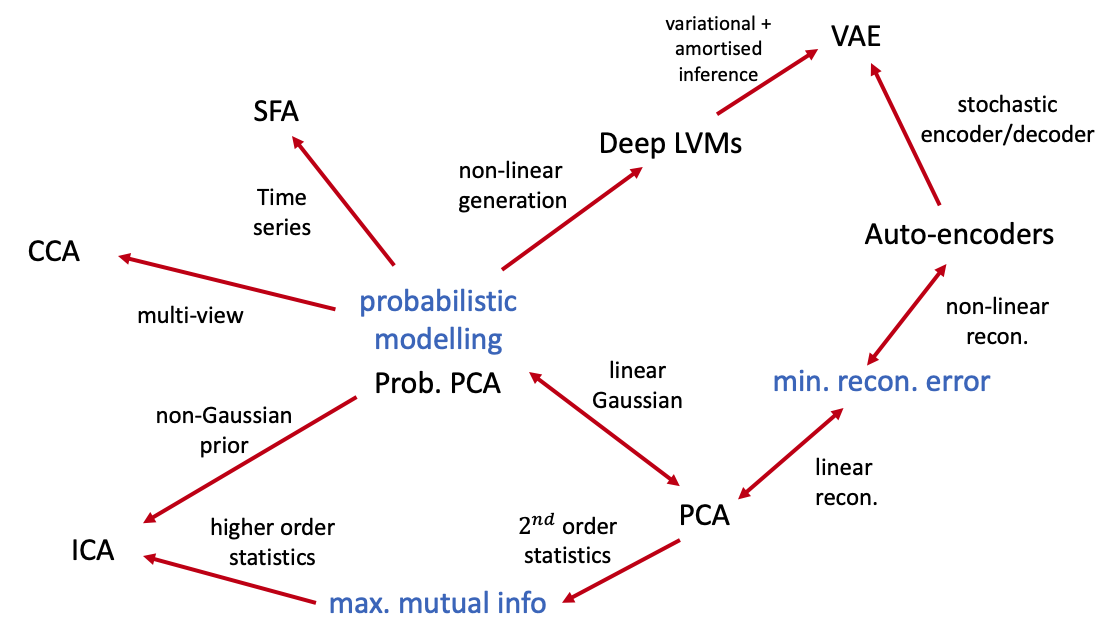
\includegraphics[width=0.9\linewidth]{figures-pca/dim_reduction_methods_vis1.png}
\end{figure}

\end{frame}

\begin{frame}{Generative models}

\begin{figure}
\centering
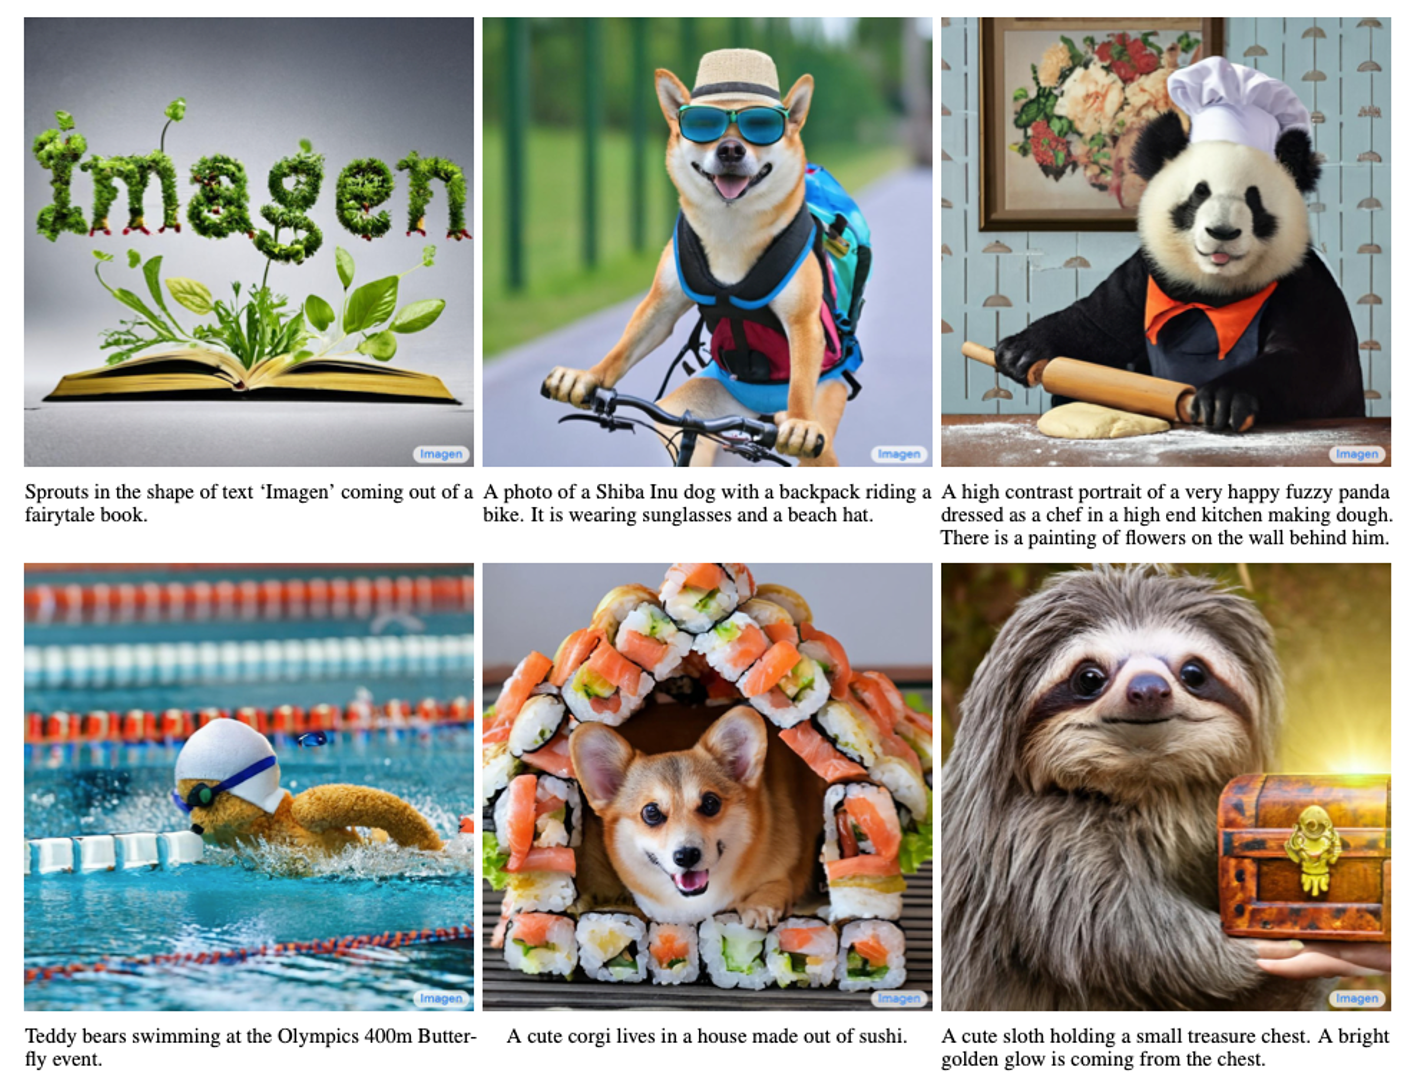
\includegraphics[width=0.75\linewidth]{figures-pca/imagen.png}
\end{figure}

\hfill
\tiny{Google's Imagen text-to-image generation model}
\end{frame}

%%%%%%%% prob PCA %%%%%%%%%

\begin{frame}{Latent Variable Models}

Data distribution: $\mathcal{D} = \{ \x_n \}_{n=1}^N, \x_n \sim \pi(\x)$

Make a generative model that generates $\x$ as follows:
$$\z \sim p_{\mparam}(\z), \quad \x \sim p_{\mparam}(\x | \z)$$

\begin{itemize}
\item $\z$: latent variable
\item $\x$: data
\item $\mparam$: model parameter to be fitted
\item if $p_{\mparam}(\x) \approx \pi(\x)$, then the model can generate realistic data
\end{itemize}

\end{frame}

\begin{frame}{Probabilistic PCA}

Data distribution: $\mathcal{D} = \{ \x_n \}_{n=1}^N, \x_n \sim \pi(\x)$

Probabilistic PCA: make a latent variable model as follows:
$$p(\z) = \mathcal{N}(\z; \bm{0}, \mathbf{I})$$
$$p_{\mparam}(\x | \z) = \mathcal{N}(\x; \BW \z + \bm{\mu}, \sigma^2 \mathbf{I})$$

\only<1>{
Sampling from this generative model:
$$\z \sim \mathcal{N}(\bm{0}, \mathbf{I}), \quad \x = \BW \z + \bm{\mu} + \sigma \bm{\epsilon}, \ \bm{\epsilon} \sim \mathcal{N}(\bm{0}, \mathbf{I}).$$

\begin{itemize}
\item model parameter: $\mparam = \{ \BW, \bm{\mu} \}$
\end{itemize}
}

\only<2->{
Marginal distribution:
\begin{equation*}
\begin{aligned}
p_{\mparam}(\x) &= \int p_{\mparam}(\x | \z) p(\z) d\z \\
\only<3>{
&= \mathcal{N}(\x; \bm{\mu}, \BW \BW^\top + \sigma^2 \mathbf{I}).
}
\end{aligned}
\end{equation*}

}

\end{frame}


\begin{frame}{Probabilistic PCA}

Data distribution: $\mathcal{D} = \{ \x_n \}_{n=1}^N, \x_n \sim \pi(\x)$

Probabilistic PCA: make a latent variable model as follows:
$$p(\z) = \mathcal{N}(\z; \bm{0}, \mathbf{I})$$
$$p_{\mparam}(\x | \z) = \mathcal{N}(\x; \BW \z + \bm{\mu}, \sigma^2 \mathbf{I})$$

Fitting $\mparam$ with Maximum Likelihood Estimation (MLE):
\begin{equation*}
\begin{aligned}
\max_{\mparam} \mathcal{L}(\mparam), \quad \mathcal{L}(\mparam) &= \frac{1}{N} \sum_{n=1}^N \log p_{\mparam}(\x_n) \\
&= \frac{1}{N} \sum_{n=1}^N \log \mathcal{N}(\x_n; \bm{\mu}, \BW \BW^\top + \sigma^2 \mathbf{I})
\end{aligned}
\end{equation*}

\end{frame}


\begin{frame}{Probabilistic PCA}

\begin{equation*}
\max_{\mparam} \mathcal{L}(\mparam), \quad \mathcal{L}(\mparam) = \frac{1}{N} \sum_{n=1}^N \log \mathcal{N}(\x_n; \bm{\mu}, \BW \BW^\top + \sigma^2 \mathbf{I}), \quad \mparam = \{ \BW, \bm{\mu} \}
\end{equation*}

Derivative of $\mathcal{L}$ w.r.t.~$\bm{\mu}$: denoting $\BC = \BW \BW^\top + \sigma^2 \mathbf{I}$
\begin{equation*}
\begin{aligned}
\frac{\partial}{\partial \bm{\mu}} \log \mathcal{N}(\x_n; \bm{\mu}, \BW \BW^\top + \sigma^2 \mathbf{I}) &= \frac{\partial}{\partial \bm{\mu}} \left( -\frac{1}{2} (\x_n - \bm{\mu})^{\top} \BC^{-1} (\x_n - \bm{\mu}) \right) \pause \\
&= (\x_n - \bm{\mu})^{\top} \BC^{-1}
\end{aligned}
\end{equation*}

$$\Rightarrow \quad \frac{\partial \mathcal{L}}{\partial \bm{\mu}} = \frac{1}{N} \sum_{n=1}^N (\x_n - \bm{\mu})^{\top} \BC^{-1}$$

Setting $\frac{\partial \mathcal{L}}{\partial \bm{\mu}} = \bm{0} \quad \Rightarrow \quad \bm{\mu}^* = \frac{1}{N} \sum_{n=1}^N \x_n$
\end{frame}

\begin{frame}{Probabilistic PCA}

\begin{equation*}
\max_{\mparam} \mathcal{L}(\mparam), \quad \mathcal{L}(\mparam) = \frac{1}{N} \sum_{n=1}^N \log \mathcal{N}(\x_n; \bm{\mu}, \BW \BW^\top + \sigma^2 \mathbf{I}), \quad \mparam = \{ \BW, \bm{\mu}, \sigma \}
\end{equation*}

Derivative of $\mathcal{L}$ w.r.t.~$\BW$: denoting $\BC = \BW \BW^\top + \sigma^2 \mathbf{I}$
\begin{equation*}
\begin{aligned}
&\frac{\partial}{\partial \BW} \log \mathcal{N}(\x_n; \bm{\mu}, \BW \BW^\top + \sigma^2 \mathbf{I}) \\
=& \frac{\partial}{\partial \BW } \left( -\frac{1}{2} (\x_n - \bm{\mu})^{\top} \BC^{-1} (\x_n - \bm{\mu}) - \frac{1}{2} \log |\BC | \right)
\end{aligned}
\end{equation*}

\begin{itemize}
\item $\BC$ depends on $\BW$, so ``chain rule'' applies
\item However, so far we've only learned about chain rule applied to scalars and vectors.
\end{itemize}

\end{frame}


\begin{frame}{Probabilistic PCA}

Applying chain rule: let $\mathcal{L}_n :=  \log \mathcal{N}(\x_n; \bm{\mu}, \BW \BW^\top + \sigma^2 \mathbf{I})$ 
\begin{itemize}
\item Chain rule for individual elements $W_{kl}$ of $\BW$:
$$\frac{\partial \mathcal{L}_n}{\partial W_{kl}} = \sum_{i, j} \frac{\partial \mathcal{L}_n}{\partial C_{ij}} \frac{\partial C_{ij}}{\partial W_{kl}}, \quad \BC = \BW \BW^\top + \sigma^2 \mathbf{I}$$
\item Calculate $\frac{\partial C_{ij}}{\partial W_{kl}}$: \pause notice $C_{ij} = \sum_{l} W_{il} W_{jl} + \sigma^2 \delta(i = j)$
\begin{footnotesize}
\begin{equation*}
\frac{\partial C_{ij}}{\partial W_{kl}} = 
\begin{cases}
0, \quad & k \notin \{i, j \} \\
W_{jl}, \quad & k = i \neq j \\
W_{il}, \quad & k = j \neq i \\
2W_{il}, \quad & k = i = j
\end{cases}
\end{equation*}
\end{footnotesize}
\pause
\item This means for fixed $k, l$:
$$\frac{\partial \mathcal{L}_n}{\partial W_{kl}} = \sum_{j} \frac{\partial \mathcal{L}_n}{\partial C_{kj}} W_{jl} + \sum_{i} \frac{\partial \mathcal{L}_n}{\partial C_{ik}} W_{il}$$
\end{itemize}

\end{frame}


\begin{frame}{Probabilistic PCA}

Applying chain rule: let $\mathcal{L}_n :=  \log \mathcal{N}(\x_n; \bm{\mu}, \BW \BW^\top + \sigma^2 \mathbf{I})$ 
\begin{itemize}
\item Chain rule for individual elements $W_{kl}$ of $\BW$:
$$\frac{\partial \mathcal{L}_n}{\partial W_{kl}} = \sum_{j} \frac{\partial \mathcal{L}_n}{\partial C_{kj}} W_{jl} + \sum_{i} \frac{\partial \mathcal{L}_n}{\partial C_{ik}} W_{il}$$
\item Writing the derivatives of $\mathcal{L}_n$ in matrix forms:
\begin{equation*}
\frac{\partial \mathcal{L}_n}{\partial \BC} =
\begin{bmatrix}
\frac{\partial \mathcal{L}_n}{\partial C_{11}} & \frac{\partial \mathcal{L}_n}{\partial C_{21}} & \hdots \\
\vdots & \ddots & \\
\frac{\partial \mathcal{L}_n}{\partial C_{1D}} & & \frac{\partial \mathcal{L}_n}{\partial C_{DD}}
\end{bmatrix}, \quad
\frac{\partial \mathcal{L}_n}{\partial \BW} =
\begin{bmatrix}
\frac{\partial \mathcal{L}_n}{\partial W_{11}} & \frac{\partial \mathcal{L}_n}{\partial W_{21}} & \hdots \\
\vdots & \ddots & \\
\frac{\partial \mathcal{L}_n}{\partial W_{1M}} & & \frac{\partial \mathcal{L}_n}{\partial W_{DM}}
\end{bmatrix} 
\end{equation*}
\only<1>{
$$\Rightarrow \quad \sum_{j} \frac{\partial \mathcal{L}_n}{\partial C_{kj}} W_{jl} = (\BW^\top)_{l \cdot} \left( \frac{\partial \mathcal{L}_n}{\partial \BC} \right)_{\cdot k}, \quad \sum_{i} \frac{\partial \mathcal{L}_n}{\partial C_{ik}} W_{il} = \left( \frac{\partial \mathcal{L}_n}{\partial \BC} \right)_{k \cdot} \BW_{\cdot l}$$
}
\only<2>{
$$\Rightarrow \quad \frac{\partial \mathcal{L}_n}{\partial \BW} = \BW^\top \left( \frac{\partial \mathcal{L}_n}{\partial \BC} + \frac{\partial \mathcal{L}_n}{\partial \BC}^\top \right)$$
}
\end{itemize}

\end{frame}


\begin{frame}{Probabilistic PCA}

$\BC = \BW \BW^\top + \sigma^2 \mathbf{I}$ is symmetric, the matrix form of the derivatives are:
$$ \frac{\partial}{\partial \BC } (\x_n - \bm{\mu})^{\top} \BC^{-1} (\x_n - \bm{\mu}) = -\BC^{-1} (\x_n - \bm{\mu}) (\x_n - \bm{\mu}) ^\top \BC^{-1}$$
$$\frac{\partial}{\partial \BC } \log |\BC| = \BC^{-1}$$
Notice that both derivatives are symmetric matrices: 
$$\frac{\partial \mathcal{L}_n}{\partial \BW} = \BW^\top \left( \frac{\partial \mathcal{L}_n}{\partial \BC} + \frac{\partial \mathcal{L}_n}{\partial \BC}^\top \right) = 2 \BW^\top \frac{\partial \mathcal{L}_n}{\partial \BC}$$

Derivative of $\mathcal{L}$ w.r.t.~$\BW$: 
\begin{equation*}
\begin{aligned}
&\frac{\partial}{\partial \BW} \log \mathcal{N}(\x_n; \bm{\mu}, \BW \BW^\top + \sigma^2 \mathbf{I}) \\
=& 2 \BW^\top \frac{\partial}{\partial \BC } \left( -\frac{1}{2} (\x_n - \bm{\mu})^{\top} \BC^{-1} (\x_n - \bm{\mu}) - \frac{1}{2} \log |\BC | \right) \\
=& \BW^\top \left( \BC^{-1} (\x_n - \bm{\mu}) (\x_n - \bm{\mu}) ^\top \BC^{-1} - \BC^{-1} \right).
\end{aligned}
\end{equation*}

\end{frame}

\begin{frame}{Probabilistic PCA}

Derivative of $\mathcal{L}$ w.r.t.~$\BW$ with $\BC = \BW \BW^\top + \sigma^2 \mathbf{I}$:
\begin{equation*}
\begin{aligned}
&\frac{\partial}{\partial \BW} \log \mathcal{N}(\x_n; \bm{\mu}, \BW \BW^\top + \sigma^2 \mathbf{I}) \\
=& 2 \BW^\top \frac{\partial}{\partial \BC } \left( -\frac{1}{2} (\x_n - \bm{\mu})^{\top} \BC^{-1} (\x_n - \bm{\mu}) - \frac{1}{2} \log |\BC | \right) \\
=& \BW^\top \left( \BC^{-1} (\x_n - \bm{\mu}) (\x_n - \bm{\mu}) ^\top \BC^{-1} - \BC^{-1} \right).
\end{aligned}
\end{equation*}

$$\Rightarrow \quad \left( \frac{\partial \mathcal{L}}{\partial \BW} \right)^\top = \BC^{-1} ( \textcolor{red}{\underbrace{\frac{1}{N} \sum_{n=1}^N (\x_n - \bm{\mu}) (\x_n - \bm{\mu}) ^\top}_{:= \BS \text{ , covariance when } \bm{\mu} = \bm{\mu}^*}} \BC^{-1} - \mathbf{I} ) \BW$$


Setting $\frac{\partial \mathcal{L}}{\partial \BW} = \bm{0} \quad \Rightarrow \quad \BW^*$ satisfies $\BS (\BW^* (\BW^*)^\top + \sigma^2 \mathbf{I})^{-1} \BW^* = \BW^*$
\end{frame}

\begin{frame}{Probabilistic PCA}

Setting $\frac{\partial \mathcal{L}}{\partial \BW} = \bm{0} \quad \Rightarrow \quad \BW^*$ satisfies $\BS (\BW^* (\BW^*)^\top + \sigma^2 \mathbf{I})^{-1} \BW^* = \BW^*$

Possible solutions for the fixed points:
\begin{itemize}
\item[1.] $\BW^* = \bm{0}$   (then $p_{\mparam^*}(\x | \z) = \mathcal{N}(\x; \bm{\mu}^*, \sigma^2 \mathbf{I})$, not interesting) 
\item[2.] Lets write down the SVD of $\BW^*$ and assume $\BW^* = \BU \Sigma \BV^\top$, \\
$\BU \in \mathbb{R}^{D \times D}, \Sigma \in \mathbb{R}^{D \times M}, \BV \in \mathbb{R}^{M \times M}$
\begin{tiny}
\begin{equation*}
\vspace{-1em}
\Sigma = 
\begin{bmatrix} 
    \sigma_{1} & 0 & \dots \\
    0 & \ddots & \\
    \vdots &        & \sigma_M \\ 
     &   &  & 0 \\
     & & & & \ddots & \\
     & & & & &  0
    \end{bmatrix} 
\quad \Rightarrow 
\Sigma \Sigma^\top + \sigma^2 \mathbf{I} = 
\begin{bmatrix} 
    \sigma_{1}^2 + \sigma^2 & 0 & \dots \\
    0 & \ddots & \\
    \vdots &        & \sigma_M^2 + \sigma^2 \\ 
     &   &  & \sigma^2 \\
     & & & & \ddots & \\
     & & & & &  \sigma^2
    \end{bmatrix} 
\end{equation*}
\end{tiny}

\end{itemize}

\end{frame}


\begin{frame}{Probabilistic PCA}

Setting $\frac{\partial \mathcal{L}}{\partial \BW} = \bm{0} \quad \Rightarrow \quad \BW^*$ satisfies $\BS (\BW^* (\BW^*)^\top + \sigma^2 \mathbf{I})^{-1} \BW^* = \BW^*$

Possible solutions for the fixed points:
\begin{itemize}
\item[1.] $\BW^* = \bm{0}$   (then $p_{\mparam^*}(\x | \z) = \mathcal{N}(\x; \bm{\mu}^*, \sigma^2 \mathbf{I})$, not interesting) 
\item[2.] Lets write down the SVD of $\BW^*$ and assume $\BW^* = \BU \Sigma \BV^\top$, \\
$\BU \in \mathbb{R}^{D \times D}, \Sigma \in \mathbb{R}^{D \times M}, \BV \in \mathbb{R}^{M \times M}$
\begin{equation*}
\begin{aligned}
\BS (\BU \Sigma \Sigma^{\top} \BU^\top + \sigma^2 \mathbf{I})^{-1} \BU \Sigma \BV^\top &= \BU \Sigma \BV^\top \\
\Rightarrow \quad \BS (\BU (\Sigma \Sigma^{\top} + \sigma^2 \mathbf{I}) \BU^\top)^{-1} \BU \Sigma \BV^\top &= \BU \Sigma \BV^\top \\
\Rightarrow \quad \BS \BU (\Sigma \Sigma^{\top} + \sigma^2 \mathbf{I})^{-1} \BU^\top \BU \Sigma \BV^\top &= \BU \Sigma \BV^\top \\
\Rightarrow \quad \BS \BU (\Sigma \Sigma^{\top} + \sigma^2 \mathbf{I})^{-1} \Sigma \BV^\top &= \BU \Sigma \BV^\top \\
\Rightarrow \quad \BS \BU (\Sigma \Sigma^{\top} + \sigma^2 \mathbf{I})^{-1} \Sigma &= \BU \Sigma
\end{aligned}
\end{equation*}
\end{itemize}

\end{frame}


\begin{frame}{Probabilistic PCA}

Setting $\frac{\partial \mathcal{L}}{\partial \BW} = \bm{0} \quad \Rightarrow \quad \BW^*$ satisfies $\BS (\BW^* (\BW^*)^\top + \sigma^2 \mathbf{I})^{-1} \BW^* = \BW^*$

Possible solutions for the fixed points:
\begin{itemize}
\item[1.] $\BW^* = \bm{0}$   (then $p_{\mparam^*}(\x | \z) = \mathcal{N}(\x; \bm{\mu}^*, \sigma^2 \mathbf{I})$, not interesting) 
\item[2.] Lets write down the SVD of $\BW^*$ and assume $\BW^* = \BU \Sigma \BV^\top$, \\
$\BU \in \mathbb{R}^{D \times D}, \Sigma \in \mathbb{R}^{D \times M}, \BV \in \mathbb{R}^{M \times M}$
%
\begin{tiny}
\begin{equation*}
\vspace{-1em}
\BS \BU 
\begin{bmatrix} 
    (\sigma_{1}^2 + \sigma^2)^{-1}\sigma_{1} & 0 & \dots \\
    0 & \ddots & \\
    \vdots &        & (\sigma_M^2 + \sigma^2)^{-1}\sigma_M \\ 
     &   &  & 0 \\
     & & & & \ddots & \\
     & & & & &  0
    \end{bmatrix} 
 = \BU
\begin{bmatrix} 
    \sigma_{1} & 0 & \dots \\
    0 & \ddots & \\
    \vdots &        & \sigma_M \\ 
     &   &  & 0 \\
     & & & & \ddots & \\
     & & & & &  0
    \end{bmatrix} 
\end{equation*}
\end{tiny}

\end{itemize}

\end{frame}


\begin{frame}{Probabilistic PCA}

Setting $\frac{\partial \mathcal{L}}{\partial \BW} = \bm{0} \quad \Rightarrow \quad \BW^*$ satisfies $\BS (\BW^* (\BW^*)^\top + \sigma^2 \mathbf{I})^{-1} \BW^* = \BW^*$

Possible solutions for the fixed points:
\begin{itemize}
\item[1.] $\BW^* = \bm{0}$   (then $p_{\mparam^*}(\x | \z) = \mathcal{N}(\x; \bm{\mu}^*, \sigma^2 \mathbf{I})$, not interesting) 
\item[2.] Lets write down the SVD of $\BW^*$ and assume $\BW^* = \BU \Sigma \BV^\top$, \\
$\BU \in \mathbb{R}^{D \times D}, \Sigma \in \mathbb{R}^{D \times M}, \BV \in \mathbb{R}^{M \times M}$
%
\begin{tiny}
\begin{equation*}
\vspace{-1em}
\BS \BU 
\begin{bmatrix} 
    1 & 0 & \dots \\
    0 & \ddots & \\
    \vdots &        & 1 \\ 
     &   &  & 0 \\
     & & & & \ddots & \\
     & & & & &  0
    \end{bmatrix} 
 = \BU
\begin{bmatrix} 
    \sigma_{1}^2 + \sigma^2 & 0 & \dots \\
    0 & \ddots & \\
    \vdots &        & \sigma_M^2 + \sigma^2 \\ 
     &   &  & 0 \\
     & & & & \ddots & \\
     & & & & &  0
    \end{bmatrix} 
\end{equation*}
\end{tiny}

\end{itemize}

Write $\BU := (\bm{u}_1, ..., \bm{u}_D)$:
$$(\BS \bm{u}_1, ..., \BS \bm{u}_M, \bm{0}, ..., \bm{0}) = ((\sigma_1^2 + \sigma^2) \bm{u}_1, ..., (\sigma_M^2 + \sigma^2) \bm{u}_M, \bm{0}, ..., \bm{0})$$


$\Rightarrow \quad$ the first $M$ columns of $\BU$ contain eigenvectors of $\BS$!

\end{frame}


\begin{frame}{Probabilistic PCA}
Setting $\frac{\partial \mathcal{L}}{\partial \BW} = \bm{0} \quad \Rightarrow \quad \BW^*$ satisfies $\BS (\BW^* (\BW^*)^\top + \sigma^2 \mathbf{I})^{-1} \BW^* = \BW^*$ \\


Possible solutions for the fixed points:
\begin{itemize}
\item[1.] $\BW^* = \bm{0}$   (then $p_{\mparam^*}(\x | \z) = \mathcal{N}(\x; \bm{\mu}^*, \sigma^2 \mathbf{I})$, not interesting) 
\item[2.] Lets write down the SVD of $\BW^*$ and assume $\BW^* = \BU \Sigma \BV^\top$, \\
$\BU \in \mathbb{R}^{D \times D}, \Sigma \in \mathbb{R}^{D \times M}, \BV \in \mathbb{R}^{M \times M}$ \\
$\Rightarrow \quad \BS \BU (\Sigma \Sigma^{\top} + \sigma^2 \mathbf{I})^{-1} \Sigma = \BU \Sigma $ \\
Then given $\BS = \BQ \Lambda \BQ^\top$, $\BQ = (\bm{q}_1, ..., \bm{q}_D)$, $\lambda_1 \geq ... \geq \lambda_D \geq 0$, 
$$\BU := (\bm{u}_{1}, ..., \bm{u}_{D}),  \bm{u}_m = \bm{q}_{i_m}, 1 \leq i_m \leq D, m = 1, ..., M$$
($\BU$ can contain any other columns for $\bm{u}_{M+1}$ to $\bm{u}_{D}$)
\end{itemize}

\end{frame}

\begin{frame}{Probabilistic PCA}
Setting $\frac{\partial \mathcal{L}}{\partial \BW} = \bm{0} \quad \Rightarrow \quad \BW^*$ satisfies $\BS (\BW^* (\BW^*)^\top + \sigma^2 \mathbf{I})^{-1} \BW^* = \BW^*$ \\


Possible solutions for the fixed points:
\begin{itemize}
\item[1.] $\BW^* = \bm{0}$   (then $p_{\mparam^*}(\x | \z) = \mathcal{N}(\x; \bm{\mu}^*, \sigma^2 \mathbf{I})$, not interesting) 
\item[2.] Lets write down the SVD of $\BW^*$ and assume $\BW^* = \BU \Sigma \BV^\top$, \\
$\BU \in \mathbb{R}^{D \times D}, \Sigma \in \mathbb{R}^{D \times M}, \BV \in \mathbb{R}^{M \times M}$ \\
Then given $\BS = \BQ \Lambda \BQ^\top$, $\lambda_1 \geq ... \geq \lambda_D \geq 0$
\begin{itemize}
	\item \alert{Exercise:} For $m = 1, ..., M$, $\Sigma_{mm} = \sqrt{\lambda_{i_m} - \sigma^2}$ if $\bm{u}_m = \bm{q}_{i_m}$
	\item \alert{Exercise:} Global maximum: $\bm{u}_m = \bm{q}_m$ for $mi = 1, ..., M$ \\
	$\Rightarrow \quad$ picking the $M$ principal components (like PCA)
\end{itemize}
\end{itemize}

\end{frame}


\begin{frame}{Probabilistic PCA}

\begin{minipage}{0.45\linewidth}
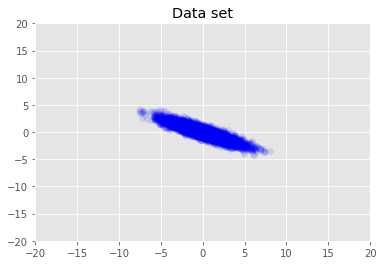
\includegraphics[width=0.9\linewidth]{figures-pca/prob_pca_data.png}

Dataset
\end{minipage}
\hfill
\begin{minipage}{0.45\linewidth}
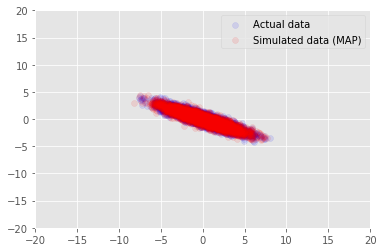
\includegraphics[width=0.9\linewidth]{figures-pca/prob_pca_samples.png}

Generate data with Prob. PCA
\end{minipage}

\vspace{3em}
\hfill
\tiny{\url{https://www.tensorflow.org/probability/examples/Probabilistic_PCA}}
\end{frame}


\begin{frame}{Extensions of Probabilistic PCA}

Probabilistic PCA: make a latent variable model as follows:
$$p(\z) = \mathcal{N}(\z; \bm{0}, \mathbf{I})$$
$$p_{\mparam}(\x | \z) = \mathcal{N}(\x; \BW \z + \bm{\mu}, \sigma^2 \mathbf{I})$$

From Probabilistic PCA to other interesting generative models:
\begin{itemize}
\item \emph{Factor analysis}: change conditional output covariance from $\sigma^2 \mathbf{I}$ to $\Psi$ (a learnable diagonal matrix)
\item \emph{Generator for a VAE}: change conditional output mean from $\BW \z + \bm{\mu}$ to $\bm{\mu}_{\mparam}(\z)$ (See Deep Learning course next term)
\item \emph{Training}: (variational) expectation maximisation \\ (See Probabilistic Inference course next term)
\end{itemize}

\end{frame}

\begin{frame}{Summary}

Probabilistic PCA
\begin{itemize}
\item One of the simplest generative model (linear generator)
\item Optimal solution closely related to PCA
\end{itemize}

One more exercise for you if you have time: \\
Derive the posterior $p_{\mparam^*}(\z | \x)$ using the optimal $\mparam^* = \{\bm{\mu}^*, \BW^* \}$

\end{frame}

%%%%%%%





\end{document}
%%% Local Variables: 
%%% mode: latex
%%% TeX-master: t
%%% End: 
